
% Template for PLoS
% Version 3.5 March 2018
%
% % % % % % % % % % % % % % % % % % % % % %
%
% -- IMPORTANT NOTE
%
% This template contains comments intended 
% to minimize problems and delays during our production 
% process. Please follow the template instructions
% whenever possible.
%
% % % % % % % % % % % % % % % % % % % % % % % 
%
% Once your paper is accepted for publication, 
% PLEASE REMOVE ALL TRACKED CHANGES in this file 
% and leave only the final text of your manuscript. 
% PLOS recommends the use of latexdiff to track changes during review, as this will help to maintain a clean tex file.
% Visit https://www.ctan.org/pkg/latexdiff?lang=en for info or contact us at latex@plos.org.
%
%
% There are no restrictions on package use within the LaTeX files except that 
% no packages listed in the template may be deleted.
%
% Please do not include colors or graphics in the text.
%
% The manuscript LaTeX source should be contained within a single file (do not use \input, \externaldocument, or similar commands).
%
% % % % % % % % % % % % % % % % % % % % % % %
%
% -- FIGURES AND TABLES
%
% Please include tables/figure captions directly after the paragraph where they are first cited in the text.
%
% DO NOT INCLUDE GRAPHICS IN YOUR MANUSCRIPT
% - Figures should be uploaded separately from your manuscript file. 
% - Figures generated using LaTeX should be extracted and removed from the PDF before submission. 
% - Figures containing multiple panels/subfigures must be combined into one image file before submission.
% For figure citations, please use "Fig" instead of "Figure".
% See http://journals.plos.org/plosone/s/figures for PLOS figure guidelines.
%
% Tables should be cell-based and may not contain:
% - spacing/line breaks within cells to alter layout or alignment
% - do not nest tabular environments (no tabular environments within tabular environments)
% - no graphics or colored text (cell background color/shading OK)
% See http://journals.plos.org/plosone/s/tables for table guidelines.
%
% For tables that exceed the width of the text column, use the adjustwidth environment as illustrated in the example table in text below.
%
% % % % % % % % % % % % % % % % % % % % % % % %
%
% -- EQUATIONS, MATH SYMBOLS, SUBSCRIPTS, AND SUPERSCRIPTS
%
% IMPORTANT
% Below are a few tips to help format your equations and other special characters according to our specifications. For more tips to help reduce the possibility of formatting errors during conversion, please see our LaTeX guidelines at http://journals.plos.org/plosone/s/latex
%
% For inline equations, please be sure to include all portions of an equation in the math environment.  For example, x$^2$ is incorrect; this should be formatted as $x^2$ (or $\mathrm{x}^2$ if the romanized font is desired).
%
% Do not include text that is not math in the math environment. For example, CO2 should be written as CO\textsubscript{2} instead of CO$_2$.
%
% Please add line breaks to long display equations when possible in order to fit size of the column. 
%
% For inline equations, please do not include punctuation (commas, etc) within the math environment unless this is part of the equation.
%
% When adding superscript or subscripts outside of brackets/braces, please group using {}.  For example, change "[U(D,E,\gamma)]^2" to "{[U(D,E,\gamma)]}^2". 
%
% Do not use \cal for caligraphic font.  Instead, use \mathcal{}
%
% % % % % % % % % % % % % % % % % % % % % % % % 
%
% Please contact latex@plos.org with any questions.
%
% % % % % % % % % % % % % % % % % % % % % % % %

\documentclass[10pt,letterpaper]{article}
\usepackage[top=0.85in,left=2.75in,footskip=0.75in]{geometry}

% amsmath and amssymb packages, useful for mathematical formulas and symbols
\usepackage{amsmath,amssymb}

% Use adjustwidth environment to exceed column width (see example table in text)
\usepackage{changepage}

% Use Unicode characters when possible
\usepackage[utf8x]{inputenc}

% textcomp package and marvosym package for additional characters
\usepackage{textcomp,marvosym}

% cite package, to clean up citations in the main text. Do not remove.
\usepackage{cite}

% Use nameref to cite supporting information files (see Supporting Information section for more info)
\usepackage{nameref,hyperref}

% line numbers
\usepackage[right]{lineno}

% ligatures disabled
\usepackage{microtype}
\DisableLigatures[f]{encoding = *, family = * }

% color can be used to apply background shading to table cells only
\usepackage[table]{xcolor}

% array package and thick rules for tables
\usepackage{array}

% create "+" rule type for thick vertical lines
\newcolumntype{+}{!{\vrule width 2pt}}

% create \thickcline for thick horizontal lines of variable length
\newlength\savedwidth
\newcommand\thickcline[1]{%
  \noalign{\global\savedwidth\arrayrulewidth\global\arrayrulewidth 2pt}%
  \cline{#1}%
  \noalign{\vskip\arrayrulewidth}%
  \noalign{\global\arrayrulewidth\savedwidth}%
}

% \thickhline command for thick horizontal lines that span the table
\newcommand\thickhline{\noalign{\global\savedwidth\arrayrulewidth\global\arrayrulewidth 2pt}%
\hline
\noalign{\global\arrayrulewidth\savedwidth}}


% Remove comment for double spacing
%\usepackage{setspace} 
%\doublespacing

% Text layout
\raggedright
\setlength{\parindent}{0.5cm}
\textwidth 5.25in 
\textheight 8.75in

% Bold the 'Figure #' in the caption and separate it from the title/caption with a period
% Captions will be left justified
\usepackage[aboveskip=1pt,labelfont=bf,labelsep=period,justification=raggedright,singlelinecheck=off]{caption}
\renewcommand{\figurename}{Fig}

% Use the PLoS provided BiBTeX style
\bibliographystyle{plos2015}

% Remove brackets from numbering in List of References
\makeatletter
\renewcommand{\@biblabel}[1]{\quad#1.}
\makeatother

% Header and Footer with logo
\usepackage{lastpage,fancyhdr,graphicx}
\usepackage{epstopdf}
%\pagestyle{myheadings}
\pagestyle{fancy}
\fancyhf{}
%\setlength{\headheight}{27.023pt}
%\lhead{\includegraphics[width=2.0in]{PLOS-submission.eps}}
\rfoot{\thepage/\pageref{LastPage}}
\renewcommand{\headrulewidth}{0pt}
\renewcommand{\footrule}{\hrule height 2pt \vspace{2mm}}
\fancyheadoffset[L]{2.25in}
\fancyfootoffset[L]{2.25in}
\lfoot{\today}

%% Include all macros below

\newcommand{\lorem}{{\bf LOREM}}
\newcommand{\ipsum}{{\bf IPSUM}}
\DeclareMathOperator{\Tr}{Tr}

%% END MACROS SECTION

% These are the packages we've added in addition to the template
\usepackage{bbold}
\usepackage{graphicx}
\usepackage{authblk}
\graphicspath{{images/}}
\usepackage[ruled,vlined]{algorithm2e}

\begin{document}
\vspace*{0.2in}

% Make title here, must ensure it's less than 250 characters
\begin{flushleft}
{\Large
\textbf\newline{The role of competition versus cooperation in microbial community coalescence}
}
\newline
\\
Pablo Lechón\textsuperscript{1,2*},
Tom Clegg\textsuperscript{2},
Jacob Cook\textsuperscript{2,3},
Thomas P. Smith\textsuperscript{2},
Samraat Pawar\textsuperscript{2}
\\
\bigskip
\textbf{1} Department of Ecology \& Evolution, University of Chicago, Chicago, IL, USA.
\\
\textbf{2} Department of Life Sciences, Imperial College London, Silwood Park, Ascot, UK
\\
\textbf{3} Centre for Integrative Systems Biology and Bioinformatics, Imperial College London, UK
\\

% As far as I (JC) can tell the main text does not reference any equations in the SM, so we don't have to check for numbering consistency
% If anyone thinks I am wrong let me know

\bigskip
*plechon@uchicago.edu

\end{flushleft}

% Abstract word limit is 300 words
\section*{Abstract}

New microbial communities often arise through the mixing of two or more separately assembled parent communities, a phenomenon that has been termed ``community coalescence". Understanding which features of complex parent communities determine the outcomes of any given coalescence event is an important challenge. While recent theoretical work has begun to elucidate the role of competition in coalescence, that of cooperation, the other key interaction type commonly seen in microbial communities, remains unclear. Here, using a general consumer-resource model we study the combined effects of competitive and cooperative interactions on the outcomes of coalescence events. We simulate coalescence between pairs of communities lying on the spectrum from competition for shared carbon resources, to cooperation through cross-feeding on leaked metabolic by-products (facilitation). Specifically, we develop novel metrics to quantify community-wide competition and cooperation levels, and show that these can predict which community dominates in pairwise coalescence events. We find that when both types of interactions are present in the parent communities, the less competitive one, which maximizes resource partitioning, contributes a higher proportion of species to the new community after coalescence, regardless of its cooperativeness. However, counter-intuitively, when competition in both parent communities is significantly weaker than facilitation, the more cooperative one is at a disadvantage during coalescence because multi-species invasions are able to disrupt established cross-feeding links. Encounters between microbial communities are becoming increasingly frequent across the globe, and there is great interest in how the coalescence of microbial communities affects environmental and human health. Our study provides new insights into the mechanisms behind microbial community coalescence, and a framework to predict outcomes based on the interaction structures of parent communities.

% Please keep the Author Summary between 150 and 200 words

\section*{Author summary}

In nature, new microbial communities often arise from the fusion of whole, previously separated communities (community coalescence). Despite the crucial role that microbial communities (and the interactions among them) play in the biosphere, the mechanisms underlying the outcomes of coalescence events remain poorly understood. Here, using a general mathematical model, we study whether and how the structure of species interactions confers an advantage upon a microbial community when it encounters another. We find that when both competition and cooperation are present, less competitive communities, which partition resources well, dominate in coalescence events. However, when competition is negligible, cooperation is in fact detrimental to coalescence success because highly cooperative communities are more susceptible to multi-species invasions. There are many potential environmental and health implications of microbial community coalescence, which will benefit from the theoretical insights that we offer here about the fundamental mechanisms underlying this phenomenon.

\linenumbers

\section*{Introduction}

Microbial communities are widespread throughout our planet \cite{Fierer2006}, from the the human gut to the deep ocean, and play a critical role in natural processes ranging from animal development and host health \cite{Huttenhower2012, McFall-Ngai2013} to biogeochemical cycles \cite{Falkowski2008}. These communities are very complex, typically harbouring hundreds of species \cite{Gilbert2014}, making them hard to characterize. Recently, DNA sequencing has allowed a high-resolution mapping of these communities, opening a niche for theoreticians and experimentalists to collaboratively decipher their complexity and assembly \cite{Costello2012,Friedman2017,Goldford2018,Goyal2018,Marsland2019,Vila2019,Estrela2020,Coyte2021,Fant2021}.

Unlike in the macroscopic world, entire, distinct microbial communities are often displaced over space and come into contact with each other due to physical (e.g., dispersal by wind or water) and biological (e.g., animal-animal interactions or leaves falling to the ground) factors \cite{Kort2014, Evans2020,Luo2020, Vass2021}. The process by which two or more communities that were previously separated join and reassemble into a new community has been termed community coalescence \cite{Rillig2015}. Despite the frequency of microbial community coalescence, the outcome of such events in terms of community structure and function remains poorly understood \cite{Rillig2016b}.

Early mathematical models of community-community invasion in animals and plants revealed that when two communities merge after barrier removal, asymmetrical dominance of one community over the other one is likely to occur \cite{Gilpin1994, Toquenaga1997}. As an explanation for this observation, it was argued that, because communities have been assembled through a history of competitive exclusion, they are likely to compete with each other as coordinated entities, rather than as a random collection of species. This result has been established more rigorously in recent theoretical work, where consumer-resource models have been used to show that in microbial community coalescence events, the winning community will be that which is capable of simultaneously depleting all resources more efficiently \cite{Tikhonov2016}. Overall, these findings suggest that communities arising from competitive species sorting exhibit sufficient ``cohesion'' to prevent successful invasions by members of other communities. 

However, empirical support for the role of competition alone in coalescence remains circumstantial, and the role of cooperation, which is commonly observed in microbial communities, remains largely unknown. For example, during coalescence in methanogenic communities, cohesive units of taxa from the community with the most efficient resource are co-selected \cite{Sierocinski2017}, and in aerobic bacterial communities, the invasion success of a given taxon is determined by its community members \cite{Lu2018}, but neither of these studies was able to establish the role of competition vs. cooperation in shaping cohesiveness, and coalescence success. The microbial communities in these experiments presumably display some degree of cooperation through cross-feeding, where leaked metabolic by-products of one species act as resources for others \cite{Hansen2007, Lawrence2012, Embree2015}. %These cross-feeding networks can vary in their particular link distribution (the architecture of the flow of resources shared between species), but also in their link weights (the fraction of consumed resources that secreted to the environment as metabolic by-products) \cite{Morris2015}. 
Indeed, several studies have suggested that a combination of competitive and cooperative interactions may determine the outcome of coalescence in microbial communities  \cite{Rivett2018, Albright2020, Castledine2020}. 

Here, we focus on the gap in our understanding of the relative importance of competition and cooperation in community coalescence, which is is largely missing. We use a consumer resource model that includes cross-feeding to assemble complex, cohesive microbial communities spanning a broad range in the competition-cooperation spectrum. Using a novel metric, we then quantify community-level competition and cooperation in the assembled communities, as well as their ``cohesiveness''. Using this metric, we then determine the relative importance of the two types of interactions on success in pairwise coalescence events. %We find that when both competition and cooperation are present, more cohesive communities out-perform competitors in coalescence events, both with and without the effects of leakage. However, when competition is negligible, we find that cohesion is detrimental to to coalescence success.

\section*{Methods}

\subsection*{Mathematical model}

We use a mathematical model based on Marsland et al \cite{Marsland2019} (see \nameref{S1_equivalence}) for microbial consumer-resource dynamics (Fig~\ref{fig:work_flow}):
\begin{align}
\begin{split}
    \frac{dn_\alpha }{dt} &= g_\alpha n_\alpha \left((1-l)\sum_j c_{\alpha j}R_j - z_\alpha \right),  \\
    \frac{dR_{j}}{dt} &= \kappa_j - \sum_\alpha n_\alpha c_{\alpha j}R_j + l\sum_{\alpha k}n_\alpha D_{kj}c_{\alpha k}R_k. 
    \end{split}
\label{eq:Model}
\end{align}
Here, $R_j$ ($j  = 1, \dots, m$) is the abundance of the $j^{th}$ resource (carbon source or substrate), and $ n_\alpha$ ($\alpha  = 1, \dots, s$) is the abundance of the $\alpha^{th}$ microbial (e.g., bacterial) species. $ \kappa_j $ is the supply rate of resource  $ j $. The growth of species $ \alpha $ is determined by the resources it harvests, which in turn depends on the resource concentration $ R_j $, and whether or not the species $ \alpha  $ uses resource $ j $ ($ c_{\alpha j} = 1 \text{ or } c_{\alpha j} = 0 $, respectively). Not all the harvested resources contribute to growth, and a fraction, $l$, leaks back to the environment (the resource pool) as metabolic by-products. $ D_{jk} $ represents the leaked proportion of resource $ j $ that is transformed into resource $ k $, and is one element of a ``stoichiometric matrix'' matrix $D$ which by definition, is a row stochastic matrix, i.e., its rows sum to 1. Each species' population uses part of its energy intake for maintenance $ z_\alpha  $, which we assume is given by:
% referenced in SM
\begin{equation}\label{eq:cost}
    z_\alpha  = \chi_0\sum_j c_{\alpha j} (1 + \epsilon).
\end{equation}
Here, $\chi_0$ is the average cost of being able to consume a given resource, the summation represents the number of resources that species $\alpha$ is able to process, and $\epsilon$ is a random fluctuation sampled from a truncated normal distribution (to ensure that $z_\alpha  > 0$). Eq~\ref{eq:cost} ensures that neither generalists nor specialists are systematically favoured during the community assembly (see \nameref{S2_cost}). The resources that remain after subtracting leakage and maintenance are transformed into biomass with a proportionality constant of $ g_\alpha  $, the value of which does not affect the results presented here.

The above model entails the following assumptions: (i) all resources contain the same amount of energy (taken to be 1 for simplicity), (ii) a type I functional response, (iii) binary consumer preferences, (iv) a shared core metabolism encoded in $D$, (v) a common leakage fractions for all species and resources, and (vi) a complex environment where all resources are externally supplied in equal amounts. We address the implications of these assumptions in the Discussion section.  

\subsection*{Competition and facilitation metrics}

Previous work suggests that during coalescence events, sets of species from the same community act as cohesive units and are selected together (ecological co-selection) \cite{Gilpin1994, Toquenaga1997, Tikhonov2016, Sierocinski2017, Lu2018}. Our goal is to quantify community-level cohesion ($\Theta$), by considering the pairwise interactions between all species in the community, and relate it to it success in coalescence events. In general we can define cohesivness of a community as the difference between its community-wide facilitation and competition,
\begin{equation}\label{eq:cohesion}
    \Theta = \mathcal{F} - \mathcal{C},
\end{equation}
where $\mathcal{C}$ and $\mathcal{F}$ are measures of community-wide competition and facilitation respectively, which we now define.

In the system described by Eqs \ref{eq:Model}, competition for resources exists because of the overlap in resource preferences (the $c_{\alpha j}$'s) between species. The realized strength of competition between species depends on the resource environment they experience, which is made up of two sources; the externally supplied resources, and the metabolic by-products generated by the community. We develop a new metric of individual pairwise competition strength that accounts for both these sources. We then measure community-level competition by taking the average competition strengths across all species pairs (see \nameref{S3_metrics} for details), that is
\begin{equation}\label{eq:competition}
    \mathcal{C} = \langle(C_a)_{\alpha \beta} + (C_b)_{\alpha \beta}\rangle_{\alpha \neq \beta}.
\end{equation}
Here, community-level competition, $\mathcal{C}$ is a unitless quantity partitioned into two components: $(C_a)_{\alpha \beta}$ measures the level of competition between species pair $(\alpha, \beta)$ for externally supplied resources, and $(C_b)_{\alpha \beta}$ the level of  competition for resources that have been leaked by species across the community. 

We define the competition for externally supplied (abiotically-generated) resources $(C_a)_{\alpha \beta}$ to be,
\begin{equation*}
	(C_a)_{\alpha\beta} = (1-l) \sum_k \tilde{\kappa}_kc_{\alpha k}c_{\beta k}.
\end{equation*}
That is, intrinsic competition between the species pair is quantified by their common resource preferences through the scalar product of their preference vectors. Interaction strength is determined by the fraction of externally supplied resources that is used for growth, $1 - l$ and the factor $\tilde{\kappa}_k$ accounts for possible differences in external supply rate between resources. 

We define competition for resources generated as metabolic by-product leakage (biotically-generated resources)  (second term in Eq~\ref{eq:competition}) as,
\begin{equation*}
	(C_b)_{\alpha\beta} = l \sum_{jk} \tilde{\kappa}_jD_{jk}\left(c_{\alpha j} + c_{\beta j}\right)c_{\alpha k}c_{\beta k}.
\end{equation*}
Here, l is the strength of competition on leaked resources (rationale behind this can be found in \nameref{S3_metrics} and \nameref{S4Fig}), and the product $ D_{jk}(c_{\alpha j} + c_{\beta j})c_{\alpha k}c_{\beta k} $ represents the necessary conditions to have effective competition for the $k^{th}$ leaked resource (see \nameref{S3_metrics} for details).

Facilitation occurs when a species leaks metabolic by-products that are used by another species. Similar to competition, we compute community-level cooperation by calculating the strengths of facilitation between individual species pairs and then averaging them across the community:
\begin{equation}
    \mathcal{F} = \langle F_{\alpha \beta} \rangle_{\alpha \neq \beta}.
\end{equation}
Here again, $\mathcal{F}$ is a unitless quantity where the facilitation between the species, $\alpha \rightarrow \beta$ is given by:
\begin{equation}\label{eq:facilitationexpanded}
F_{\alpha \beta} = l \sum_{jk} \tilde{\kappa}_jc_{\alpha j}D_{jk}c_{\beta k},
\end{equation}
where $l$ is the strength of cooperative links, and the term $c_{\alpha j}D_{jk}c_{\beta k}$ represents the necessary condition to establish a cooperative link (see \nameref{S3_metrics} for further details).

\subsection*{Simulations}

Fig~\ref{fig:work_flow} presents an overview of our simulation methodology. The matrix implementation used in the actual simulations is described in the \nameref{S4_matrices}. %For the parameter values used in the simulations, see \nameref{S1_Appendix}.
% All figures have to be placed after the first paragraph they are referenced
\begin{figure}[t]
\begin{adjustwidth}{-2.2in}{0in}
    \centering
    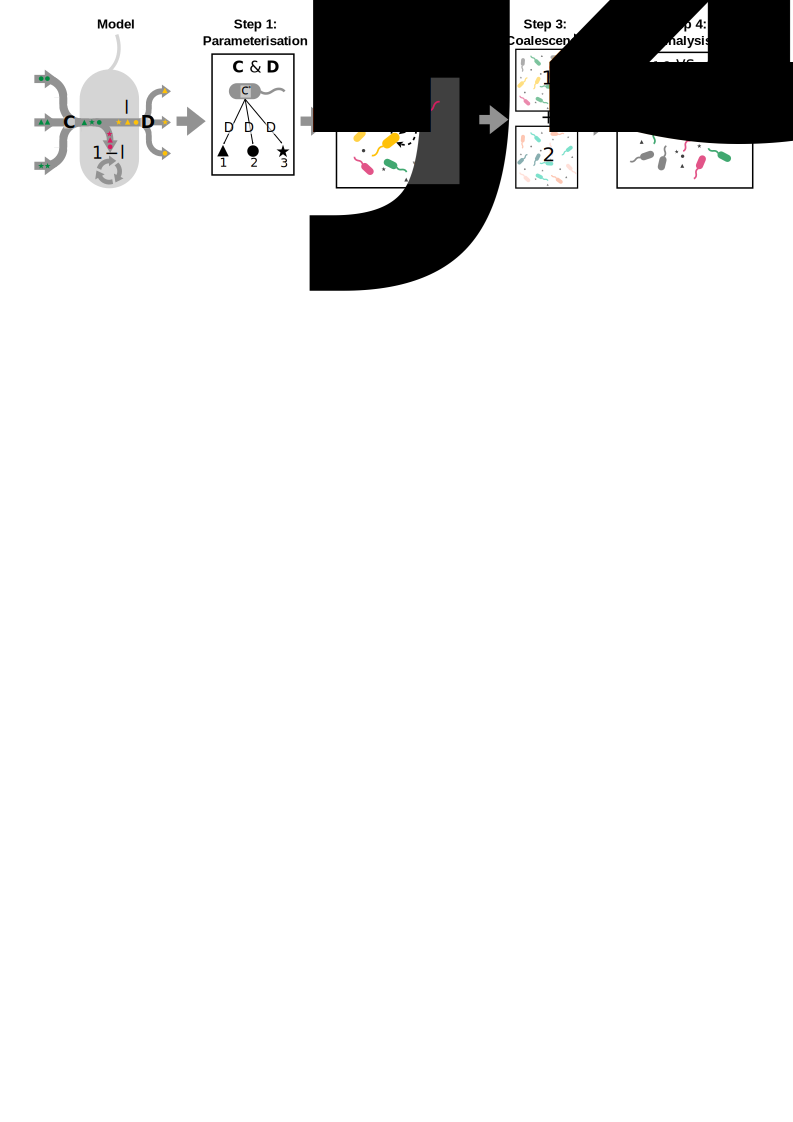
\includegraphics[width=1.40\columnwidth]{hand_plot_flow.pdf}
    \vspace{15pt}
    \caption{\textbf{Overview of the coalescence modelling methodology.} \textbf{Step 1}. The metabolic preferences $C$, and the metabolic matrix $D$, are sampled for each community under just the assumption of preferential feeding (Fig~\ref{fig:three_sampling_scenarios}B, and E), or both the latter and the assumption of structure in guilds (Fig~\ref{fig:three_sampling_scenarios}B\&C, and \ref{fig:three_sampling_scenarios}E\&F) . \textbf{Step 2}. Dynamics of the system are allowed to play out (Eqs~\ref{eq:Model}) until equilibrium is reached.\textbf{ Step 3}. Assembled communities are randomly paired up and each hybrid community re-run to steady state. \textbf{Step 4}. The contribution of each community to the final mix is analyzed ($S_{1, 2}$, Eq~\ref{eq:similarity}) as a function of the cohesion in the original pair of communities ($\Delta\Theta$, Eq~\ref{eq:cohesion}).}
    \label{fig:work_flow}
\end{adjustwidth}
\end{figure}


\subsubsection*{Step 1: Parameterisation}\label{Step1}\vspace{-5pt}

We first assemble parent communities with their interactions lying on a spectrum of competition to cooperation. To this end, for each parent community, resource preferences and secretion parameters (the $ c_{\alpha j} $'s and $ D_{jk} $'s, respectively) of $s = 60$ consumer species are sampled from random distributions, but with certain constraints in order to modulate the competition and facilitation levels (cohesiveness) achieved at steady state.

\textit{Modulating competition and facilitation levels}.  We use an iterative procedure to impose a specific level of competition by increasing or decreasing niche similarity between consumers (see \nameref{S5_preferential}). In this procedure, resource preferences of single species are assigned iteratively by re-evaluating the probability that species $\alpha$ samples resource $j$, given by
\begin{equation}\label{eq:sampling_probability}
	p_{\alpha j}= (1-k_c) \frac{1}{m}  + k_c \tilde{d}_{\alpha  -1j},
\end{equation}
where $m$ is the number of resource types, $\tilde{d}_{\alpha  -1j}$ is the normalized cumulative demand of resource $j$ at iteration $\alpha - 1$, and $k_c$ is the competitiveness factor (see \nameref{S5_preferential} for details). In each step of the iteration, the sampling probability of each resource by a given consumer is changed according to the demand on it such that highly-demanded resources are more likely to be sampled in the next step (``preferential feeding''). Note that $k_c$ modulates how much consumers prefer highly-demanded resources, such that when $k_c = 0$, the sampling is uniformly random (Fig~\ref{fig:three_sampling_scenarios}A); as $k_c \rightarrow 1$, the feeding becomes increasingly preferential (Fig~\ref{fig:three_sampling_scenarios}B).

% All figures should be placed immediately after the first paragraph they were referenced in
\begin{figure}[t]
\begin{adjustwidth}{-1.5in}{0in}
	\centering
	\includegraphics[width=1.2\columnwidth]{sampling_scenarios.pdf}
	\caption{\textbf{Examples of differently structured preference ($C$) and metabolic ($D$) matrices}. These have been generated with different combinations of the competition and facilitation parameters $k_c$, $K_c$, $k_f$, and $K_f$ in systems of 60 resource types and 60 consumer species. In the metabolic matrices (D--F), lighter colours indicate higher values (resource fractions secreted). {\bf A \& D}: Purely random matrices, where  all the four parameters are 0. {\bf B \& E}: As $k_c$ and $k_f$ are increased the regime moves towards greater preferential feeding, where more demanded resources are more likely to be consumed (increase of $k_c$), but also secreted at higher fractions (increase of $k_f$). {\bf C \& F}: Instead, if $K_c$ and $K_f$ are increased, the regime moves towards more structured resource use, where species are more likely to consume resources from their preferred resource class (a resource guild) (increase in $K_c$), and leak higher fractions of resources that do not belong to their preferred resource class (increase in $K_f$).}
	\label{fig:three_sampling_scenarios}
\end{adjustwidth}
\end{figure}

The facilitation level of the community depends on the topology of metabolic by-product secretion encoded in the community metabolic matrix $ D $ (Fig~\ref{fig:three_sampling_scenarios}D), which is specified such that the resources that are highly demanded are also secreted in large fractions  (Fig~\ref{fig:three_sampling_scenarios}E, and see \nameref{S5_preferential} for details).\\

\textit{Introducing structure in guilds}. 
%Above, we imposed a preferential feeding structure on the community's resource consumption and processing that allowed us to modulate the levels of competition and facilitation. However, increasing levels of facilitation by greater leaking of highly-demanded resources only decreases competition for externally-supplied (abiotically-generated) resources, leaving competition for leaked (biotically-generated) resources unchanged.
Many microbial communities have been found to be taxonomically variable, but functionally stable \cite{Louca2018, Enke2019}, suggesting that many different species belonging to the same guild would be able to perform similar metabolic tasks, rendering them functionally redundant. Theoretical studies support these observations \cite{Goldford2018, Fant2021, Marsland2020}. Consequent with this pervasive feature in microbial assemblages, we add further strucutre in the form of "guilds" to the matrices $C$ and $D$ by partitioning the resources into different classes, and constraining consumers to feed on a preferred class, but leak to any other. Adding this structure yields two levels of cooperation: inter-guild facilitation between consumers preferring distinct resource classes, and intra-guild facilitation due to the previously-imposed preferential feeding (imagine superimposing Figs~\ref{fig:three_sampling_scenarios}B\&C, and Figs~\ref{fig:three_sampling_scenarios}E\&F).
%In order to decouple facilitation from competition on biotically-generated resources, we need to ensure that the resources that species' consume are not the same as the ones they leak. That is, we need to increase species' niche complementarity among functional consumer groups (or guilds), as has been observed in real systems \cite{Goldford2018, Marsland2020}. 
Resource preferences are now assigned similarly to the unstructured preferential feeding above, except that the probability that species $\alpha_A$ (which feeds preferably on resource class $A$) is now weighted up or down depending on whether resource $j$ belongs in $A$, or not, respectively (Fig~\ref{fig:three_sampling_scenarios}C, derivation in \nameref{S6_classes}), as:
% Referred to in SM
\begin{equation}\label{eq:general_sampling}
    p^A_{\alpha j} = 
     \begin{cases}
        \dfrac{1}{\mathcal{A}}\left(1 + K_c(N_c - 1)\right) \Big(\dfrac{1}{m}\left(1-k_c\right) + \tilde{d}_{\alpha - 1 j}k_c\Big) & \text{if } j \in A \\[10pt]
        \dfrac{1}{m}(1-K_c) & \text{otherwise}.
     \end{cases}
\end{equation}
Here $\mathcal{A}$ is a normalization constant ensuring that the probabilities sum to 1. The magnitude of this effect is given by the constant $K_c$, which controls the amount of resource guild structure in $C$.

The metabolic matrix $D$ is constructed such that the fraction of by-product $k$ leaked is lower if that resource belongs to the same class as the consumed resource $j$ (elements within block-diagonals of $D$), and higher otherwise (off-block diagonal elements of $D$) (Fig~\ref{fig:three_sampling_scenarios}F). The prominence of this structure in the matrix is given by the inter-guild facilitation factor $K_f$ (see \nameref{S6_classes} for details).

\subsubsection*{Step 2: Assembly of parent communities}\vspace{-5pt}

After parameterisation, dynamics of each parent community are allowed to play out in an environment with 60 consumer species and resource types ($s = m = 60$), according to Eqs \ref{eq:Model} till it reaches steady state. We assemble parent communities under both, just preferential feeding and resource guild-structured plus preferential feeding parameterisations of the metabolic matrices. Within each of the two sets, we perform 100 random assembly processes at every point of a parameter grid that encompasses all possible combinations of $l = k_c = k_f = [0,...,0.9]$, and $K_c = K_f = 0$ or $K_c = K_f = 0.9$ depending if we are on the first, or second sampling scenarios, respectively. Further details of the assembly simulations are in \nameref{S7_assembly}.

\subsubsection*{Step 3: Coalescence}\vspace{-5pt}

Random pairs of assembled communities lying on the spectrum of competition to cooperation are mixed and the hybrid community re-run to steady state. Each such coalescence event is simulated by mixing the two parent communities in fresh ``media'' (all resources are set to the initial concentrations before assembly) (see \nameref{S7_assembly} for further details). For each value of leakage, we simulate 2 $\cdot 10^4$ such coalescence events.

\subsubsection*{Step 4: Analysis}\vspace{-5pt}

After coalescence, at steady state of the new (coalesced) community, we analyse the contribution of each parent community to species' presence/absence in the coalesced community, and how this contribution depends on the nature of interactions (cohesiveness) in the parent communities ($\Theta$; Eq \ref{eq:cohesion}). That is, the cohesion values of each community ($\Theta_1$ and $\Theta_2$) are recorded before coalescence. We propose the following measure of similarity of the coalesced community to the two parents (indexed by 1 and 2) (a measure of parent community dominance):
\begin{equation}\label{eq:similarity}
    S_{1,2} = \vec{p_f}\cdot\left(\dfrac{1}{r_1} \vec{p_1} - \dfrac{1}{r_2}\vec{p_2}\right), 
\end{equation}
where $\vec{p_f}$, $\vec{p_1}$, and $\vec{p_2}$ are $(s_1 + s_2)$--dimensional vectors of species presence-absence in the post-coalescent, parent community 1, and 2, respectively, with $r_1$ and $r_2$ the species richness values of the parent communities 1 and 2, respectively (calculated as $r_i = \sum \vec{p_i}$). If $S_{1,2} = 1$, the coalesced community is identical to parent community 1, and if $S = -1$, it is identical to parent community 2. This measure is richness independent, allowing us to mix communities with different richness levels, avoiding bias in similarity towards the richer one.

\section*{Results}

\subsection*{Minimizing competition ensures coalescence success}

We first simulate coalescence between pairs of communities assembled under preferential feeding only (Fig~\ref{fig:three_sampling_scenarios}B, E). Under this scenario, we calculate the effective community leakage matrix $CD$ for one representative exapmle community (Fig~\ref{fig:assumption1}A). The element $(CD)_{\alpha k}$ accounts fo the total leakage of resource $k$ by species $\alpha$  given $\alpha$'s consumption preferences. Consequently, this value will be higher for generalists. Reordering columns and rows of this matrix according to the dominant eigenvector (that associated with the largest eigenvalue), we find that leakage matrix has nested structure, that is, generalists are facilitators, since they are the main contributors more demanded resources. Using these communities in the coalescence experiments, we find that coalesced communities tend to be more similar to their more cohesive parent for all leakage values (Fig~\ref{fig:assumption1}B). With low leakage, facilitation is negligible (blue line in Fig~\ref{fig:assumption1}C), and competition is mainly for abiotically-generated resources (dashed line in Fig~\ref{fig:assumption1}C). Thus, in this regime, being more cohesive is equivalent to being less competitive. Therefore, in the low leakage regime, communities that minimize competition succeed in coalescence events. This trend remains even at the highest value of leakage, where facilitation is slightly larger than competition (now mainly for leaked resources) on average. This indicates that with purely preferential feeding, (minimising) competition drives the outcome of community coalescence, overriding the effects of facilitation. Previous work has linked success in  coalescence to effective resource usage. To test this hypothesis, we plot  resource abundance at equilibrium as a function of intrinsic cohesion of the community (Fig~\ref{fig:assumption1}D), which is given by
\begin{equation}
    \hat{\Theta} = \frac{1}{l}(F - C_b) - \frac{1}{1-l}C_a,
\end{equation}
and accounts only for the cohesion structure, leaving out the strength of the links (allowing comparison between different values of leakage). We find that more cohesive communities deplete resources more efficiently.
\begin{figure}[t]
\begin{adjustwidth}{-1.5in}{0in}
    \centering \includegraphics[width=1.3\columnwidth]{images/figure_3_compiled.pdf}
    \caption{\textbf{Community coalescence with preferential feeding.} {\bf A}: Example of the secretion matrix of $(C D)_{\alpha k}$'s, the total leakage of resource $k$ by an individual of species $\alpha$. Columns and rows have been reordered, revealing a nested structure where a portion of species (lighter top rows) leak the majority of the highly-demanded resources (lighter left columns). {\bf B}: The post-coalescence community is more similar to its more cohesive parent. Shown is binned mean (20 bins) over communities with similar parent cohesion difference $\Theta_1  - \Theta_2$ (solid line) $\pm$ 1 standard deviation (shaded) for the three leakage values. {\bf C}: Community-level competition $\mathcal{C}$ (dark red) and facilitation $\mathcal{F}$ (blue) averaged across simulations for each leakage value. Competition for abiotically-generated resources ($C_a$) decreases and that for biotically-generated resources ($C_b$) increases with leakage, with total competition remaining consistently high throughout. Facilitation, on the other hand, increases linearly with leakage. {\bf D}: Total resource abundance at equilibrium is negatively correlated with intrinsic cohesion, confirming that more cohesive communities are better at depleting resources to the lowest concentration.}
    \label{fig:assumption1}
\end{adjustwidth}
\end{figure}

% Figures placed immediately after the first paragraph they are referred to
\begin{figure}[t]
\begin{adjustwidth}{-1.5in}{0in}
    \centering \includegraphics[width=1.3\columnwidth]{images/figure_4_compiled.pdf}
    \caption{\textbf{Community coalescence with resource guilds present.} {\bf A}: Example of a secretion matrix with resource guild structure in addition to preferential feeding. {\bf B}: Community-level competition ($\mathcal{C}$) and facilitation ($\mathcal{F}$) averaged across simulations for different levels of leakage. For low values of leakage, competition for abiotically-generated resources ($C_a$; dashed decreasing line) dominates, and for high values of leakage facilitation ($F$) is the important term. Competition for biotically-generated resources ($C_b$; dashed increasing line) is consistently low due to the resource guild structure imposed on the secretion matrix. {\bf C}: Parent community dominance is positively correlated with $\Delta \Theta$ for low values of leakage, when $\mathcal{C} > \mathcal{F}$ (cf. Eq \ref{eq:cohesion}); but negatively correlated with $\Delta \Theta$ for high values of leakage, when $\mathcal{C} < \mathcal{F}$. {\bf D}: The difference in average intrinsic facilitation between extinct species, loosing parent community, and post-coalescence community, increases with leakage, suggesting that in more cooperative communities, facilitation links are being intercepted by invading species}
    \label{fig:assumption2}
\end{adjustwidth}
\end{figure}

\subsection*{Guild structure renders cooperation detrimental}

 Imposing this resource guild structure results in the term $C_b$ in Eq~\ref{eq:competition} becoming effectively very low, bringing out a new regime at high $l$ values where $\mathcal{C} << \mathcal{F}$ (Fig~\ref{fig:assumption2}B). The coalescence simulations are now run on such pairs of parent communities. We find that in the low leakage regime, where competition is present, we recover the previous result (yellow and red lines in Fig \ref{fig:assumption2}C) with preferential feeding only (Fig \ref{fig:assumption1}B). In the high leakage regime, competition is negligible, so being more cohesive is equivalent to having higher levels of facilitation. In this scenario, we find that cohesion is negatively correlated with coalescence success, that is, more facilitative communities perform poorly in coalescence events (black line, Fig~\ref{fig:assumption2}C), and are are easily invaded by a randomly-picked invading community. One experimentally supported explanation for this observation is that multi-species invasions disrupt cooperative links \cite{Machado, Altieri2010, Li2019}. To test whether or not this mechanism is responsible for our observation, we measure the average facilitation in the mixed and loosing communities, as well as in the group of species that go extinct during the coalescence event, across all simulations at each leakage value (Fig~\ref{fig:assumption2}D). The result confirms our intuition, since we find that the species that go extinct engage in stronger cooperative links than those of the post-coalescence community, and even the ones of the loosing community for very high values of leakage. Note that the y-axis in Fig~\ref{fig:assumption2}D is leakage independent, and therefore it is only measuring the facilitation topology, that is, the amount of cooperative links, independently of their flux ($l$, recall Eq~\ref{eq:facilitationexpanded} )
 
\section*{Discussion}

New microbial communities often emerge through community coalescence  \cite{Rillig2015}. Previous studies have focused on the emergent cohesiveness between coalescing communities, and explained it in terms of resource depletion efficiency \cite{Gilpin1994, Toquenaga1997, Livingston2013, Tikhonov2016, Sierocinski2017, Tikhonov2017, Lu2018, Rivett2018}. Our findings confirm these results, and offer new ones, while framing them in a broader context by considering explicitly the effect of competition for resources and the cooperation arising through facilitation by cross-feeding on metabolic by-products (resource leakage). In particular, we find that the balance between competition and facilitation can substantially change the outcome of coalescence events, as has been suggested recently \cite{Castledine2020}. Minimizing competition turns out to be the dominant driving force of coalescence processes, while minimizing cooperation is a secondary effect that arises when competition for resources is brought to a minimum.

In the work of \cite{Tikhonov2016}, the cohesiveness displayed by coalescing communities in the absence of cooperative interactions was explained in terms of effective resource depletion. This allowed the winning community to engineer an environment more favorable for itself than for the losing community, which was partially or completely displaced. The latter theoretical prediction has been experimentally verified in methanogenic communities \cite{Sierocinski2017}, which are characterized by a dense metabolic cross-feeding network. However, we cannot help to question this claim: how is it possible that a minimal theoretical setting built exclusively around competition can explain the complex reality of coalescence events in the presence of syntrophy?

In this work we presented a theoretical framework that incorporates the intricate cross-feeding topology displayed by microbial communities and more realistically reconciles theory with observations. The previous theoretical result suggesting that in a coalescent event, ``the winning [more cohesive] community is the one that is most efficient at depleting all substrates simultaneously", appears here as a particular case of a more general description. In this work cohesiveness is not defined in terms of resource depletion efficacy, but rather in terms of minimizing competition and maximizing cooperation. Reassuringly, the emerging pattern at $l\approx0$, obtained here through our interaction-dependent cohesion measure (yellow line in Fig~\ref{fig:assumption1}B), parallels that emerging in  \cite{Tikhonov2016} through the resource-depletion-dependent cohesion measure. Thus, considering also that in the purely competitive regime, our model collapses  to the one presented in \cite{Tikhonov2016} (see \nameref{S1_equivalence}), it appears that resource use efficiency is a consequence of minimizing competition.

%New microbial communities often emerge through community coalescence  \cite{Rillig2015}. Previous studies have focused on coalescence as an outcome of competition between two parent communities, each behaving as coherent whole \cite{Gilpin1994, Toquenaga1997, Livingston2013, Tikhonov2016, Sierocinski2017, Tikhonov2017, Lu2018, Rivett2018}. Our findings generalize these results to include cooperation arising through facilitation by cross-feeding on metabolic by-products (resource leakage). In particular, we find that the balance between competition and facilitation can substantially change the outcome of coalescence events, as has been suggested recently \cite{Castledine2020}. ...

%In the theoretical study by Tikhonov \cite{Tikhonov2016}, greater cohesiveness in coalescing communities resulted in greater resource depletion in the absence of cooperative interactions. This cohesiveness was essentially the result of minimizing competition by resource (niche) partitioning, and allowed the community that dominated at the end of coalescence to engineer an environment more favorable for itself than for the losing community, which was partially or completely displaced. Thus, the success of any one species during a coalescence event depends on the community-level `fitness' of its parent community more than its intrinsic fitness, {\it per se}. In our work, cohesiveness is not defined in terms of resource depletion efficacy, but rather in terms of lying on a spectrum of minimizing competition to maximizing cooperation (the measure $\Theta$; Eq \ref{eq:cohesion}). In \nameref{S1_equivalence}, we show that in the purely competitive regime (when leakage $l\approx0$), our model collapses to Tikhonov \cite{Tikhonov2016}'s model. Thus, our interaction-dependent cohesion measure (yellow line in Fig~\ref{fig:assumption1}B) is analogous to the resource-depletion-dependent cohesion measure developed by Tikhonov \cite{Tikhonov2016}.  ...it appears that resource use efficiency is a consequence of minimizing competition.

The consistency of the trend in Fig~\ref{fig:assumption1}B across the whole leakage range suggests that minimising competition is the main factor driving the outcome of community coalescence even in the presence of cooperation. When $l > 0$, high competition levels prevailed, but were taking place in an altered environment, one engineered by a community that both consumed and secreted resources. Ultimately, competition for leaked resources exists because the species are secreting resources necessary for their own growth. While this might seem disadvantageous and thus unrealistic at first, leaking essential resources is an observed phenomenon in many microbial systems \cite{Paczia2012, Silva2015}, and may be advantageous as a ``flux control'' mechanism employed by individual cells to promote growth in crowded environments \cite{Yamagishi2020, Yamagishi2020a}. Overall, these findings extend the results of previous theoretical studies to accommodate metabolic interdependence (cross-feeding); an essential feature of real microbial communities \cite{Machado, Pascual-Garcia2020}.  Our results also provide theoretical, mechanistic insights into empirical studies that have demonstrated the importance of cross-feeding interactions on coalescence \cite{Sierocinski2017}.

Many microbial communities have been found to be taxonomically variable, but functionally stable \cite{Louca2018, Enke2019}, suggesting that many different species belonging to the same guild would be able to perform similar metabolic tasks, rendering them functionally redundant. This observation is supported by recent theoretical studies, which recognize that stable and (sometimes even) analytically predictable structure in guilds arise when communities assemble in complex environments \cite{Goldford2018, Marsland2019, Marsland2020, Fant2021}. Consequent with this pervasive feature in microbial assemblages, we performed a second set of coalescence simulations after adding a guild structure to our system. Upon this new structure, we saw a new regime emerge where the community-level cooperation was significantly higher than competition for high values of leakage. In this regime, multi-species invasions were found to easily disrupt facilitative links in the more cooperative community. This result is experimentally supported by several studies \cite{Altieri2010, Li2019, Machado} which recognize that strong cooperative links are susceptible to be intercepted by species invasions. Nonetheless, recent \textit{in-silico} results of single species invasions on microbial communities have found that cooperative communities are more resistant to invasions than their competitive counterparts \cite{Kurkjian2021}. The apparent contradiction between this finding and our own suggests that invasions in the context of complex communities  cannot be understood from the study of single species invasions \cite{Sierocinki2021}.

Throughout this work, we assumed that all resources were supplied, and at a fixed rate. Removing environmental fluctuations, ensured that the effects we observed were only due to the species interactions, allowing us to pinpoint their role separately. While this assumption may be sensible in some cases \cite{Acosta2015}, it is an oversimplification in others \cite{Albright2020}. Extending this theoretical framework to study the effects of resource supply variation, e.g., by allowing substrate diversification from a single supplied resource \cite{Goldford2018, Marsland2019}, is a promising direction for future research. In such case, we expect that only the cooperative links necessary to diversify the supplied carbon source will persist upon coalescence events, but above that threshold, the results presented here would be recovered. The resource dynamics where further simplified in this work by assuming a type-I functional response. This is not expected to change our results substantially, since our simulations are performed at steady state, where all three types of functional responses behave the same. Given the heavy simulation based approach taken here, assuming a core metabolism and leakage common to the whole community, made the dynamics computationally tractable, while ensuring that the system was not far away from real communities \cite{Marsland2019, Marsland2020}.

The pairs of coalescing communities in this work were drawn with no richness restrictions, that is, communities with different species richness were allowed to compete. Consequently, the results reported here are independent of the species richness of the mixed communities. Interestingly, several previous studies have pointed to microbial community diversity as an important factor driving resource use efficiency and, therefore, determining community resistance against biotic and abiotic perturbations \cite{Girvan2005, Eisenhauer2012, Maron2018}. These observations do not necessarily contradict the results reported here. Instead, our findings suggest that community interactions may be a more fundamental mechanism explaining the response of communities to environmental and biotic perturbations, and that biodiversity is rather a consequence of the underlying community interaction network. It is not surprising that empirical studies usually focus on biodiversity's influence on community stability (the ``diversity-stability'' relationship) rather than of community interactions, since the latter is much harder to measure than the former. Understanding biodiversity as an emergent property of the interaction network topology in a microbial community is a promising line of research \cite{Ratzke2020a}.
%, particularly in the context of climate change/agriculture/health (REFERENCE(S)).

% The only interactions considered here were cooperation through metabolic facilitation and competition. However, microbial inter-relations are more complex than just a binary classification \cite{Pacheco2019}, often involving the release of antimicrobial compounds, end-product inhibition, predation, or interactions with spatial dependencies, an aspect that was also omitted here. 

Encounters between microbial communities  are becoming increasingly frequent \cite{Seebens2017}, and mixing of whole microbial communities is gaining popularity for bio-engineering \cite{Rillig2016}, soil restoration \cite{Calderon2017}, faecal microbiota transplantation \cite{Wang2019, Wilson2019}, and the use of probiotics \cite{Lindemann2016}. We present a framework which relates the nature of species interaction in microbial communities to the outcome of community coalescence events. Although more work is required to bridge the gap between theory and empirical observations, this study constitutes a key step in that direction.

\section*{Supporting information}

% CITE SI USING (For more information, see \nameref{S1_Appendix}.)

% Include only the SI item label in the paragraph heading. Use the \nameref{label} command to cite SI items in the text.
\paragraph*{Supporting text section 1}\textbf{--  Relationship with other consumer resource models.}
\label{S1_equivalence}
\paragraph*{Supporting text section 2}\textbf{--  Cost function.}
\label{S2_cost}
\paragraph*{Supporting text section 3}\textbf{--  Metrics.}
\label{S3_metrics}
\paragraph*{Supporting text section 4}\textbf{--  Preferential feeding.}
\label{S5_preferential}
\paragraph*{Supporting text section 5}\textbf{--  Adding structure in resource classes.}
\label{S6_classes}
\paragraph*{Supporting text section 6}\textbf{--  Community Assembly.}
\label{S7_assembly}
\paragraph*{Supporting text section 7}\textbf{--  Matrix representations.}
\label{S4_matrices}
\paragraph*{S4 Fig}\textbf{--  Mechanism of resource recycling}
\label{S4Fig}
\paragraph*{S8 Fig}\textbf{--  Heat-maps for each value of l of the average richness r as a function of $k_c$ and $k_f$.}
\label{S8_Fig}

\section*{Author Contributions}
\textbf{Conceptualization:} Pablo Lechón, Tom Clegg, Jacob Cook, Thomas P. Smith, Samraat Pawar\\[10pt]
\hspace{-14pt}\textbf{Formal Analysis:} Pablo Lechón \\[10pt]
\hspace{-14pt}\textbf{Methodology} Pablo Lechón \\[10pt]
\hspace{-14pt}\textbf{Software} Pablo Lechón \\[10pt]
\hspace{-14pt}\textbf{Visualization:} Pablo Lechón \\[10pt]
\hspace{-14pt}\textbf{Writing – Original Draft Preparation:} Pablo Lechón \\[10pt]
\hspace{-14pt}\textbf{Writing – Review \& Editing:} Pablo Lechón, Jacob Cook, Thomas P. Smith, Tom Clegg, Samraat Pawar. \\[10pt]
\hspace{-14pt}\textbf{Funding Acquisition:} Samraat Pawar \\[10pt]

%\section*{Acknowledgments}
%THANK PEOPLE

\nolinenumbers

\begin{thebibliography}{10}

\bibitem{Fierer2006}
Fierer N, Jackson RB.
\newblock {The diversity and biogeography of soil bacterial communities}.
\newblock Proceedings of the National Academy of Sciences of the United States
  of America. 2006;103(3):626--631.
\newblock doi:{10.1073/pnas.0507535103}.

\bibitem{Huttenhower2012}
Huttenhower C, Gevers D, Knight R, Al E.
\newblock {Structure, function and diversity of the healthy human microbiome}.
\newblock Nature. 2012;486(7402):207–214.
\newblock doi:{10.1038/nature11234}.

\bibitem{McFall-Ngai2013}
McFall-Ngai M, Hadfield MG, Bosch TCG, Carey HV, Domazet-Lo{\v{s}}o T, Douglas
  AE, et~al.
\newblock {Animals in a bacterial world, a new imperative for the life sciences}.
\newblock Proceedings of the National Academy of Sciences of the United States of America. 2013;110(9):3229--3236.
\newblock doi:{10.1073/pnas.1218525110}.

\bibitem{Falkowski2008}
Falkowski PG, Fenchel T, Delong EF.
\newblock {The microbial engines that drive earth's biogeochemical cycles}.
\newblock Science. 2008;320(5879):1034--1039.
\newblock doi:{10.1126/science.1153213}.

\bibitem{Gilbert2014}
Gilbert JA, Jansson JK, Knight R.
\newblock {The Earth Microbiome project: Successes and aspirations}.
\newblock BMC Biology. 2014;12(69):12915--014.
\newblock doi:{10.1186/s12915-014-0069-1}.

\bibitem{Marsland2019}
Marsland R, Cui W, Goldford J, Sanchez A, Korolev K, Mehta P.
\newblock {Available energy fluxes drive a transition in the diversity, stability, and functional structure of microbial communities}.
\newblock PLoS Computational Biology. 2019;15(2):e1006793. doi:
  10.1371/journal.pcbi.1006793.
\newblock doi:{10.1371/journal.pcbi.1006793}.

\bibitem{Goldford2018}
Goldford JE, Lu N, Baji{\'{c}} D, Estrela S, Tikhonov M, Sanchez-Gorostiaga A,
  et~al.
\newblock {Emergent simplicity in microbial community assembly}.
\newblock Science. 2018;361(6401):469--474.
\newblock doi:{10.1126/science.aat1168}.

\bibitem{Goyal2018}
Goyal A, Maslov S.
\newblock {Diversity, Stability, and Reproducibility in Stochastically
  Assembled Microbial Ecosystems}.
\newblock Physical Review Letters. 2018;120(15):158102. doi:
  10.1103/PhysRevLett.120.158102.
\newblock doi:{10.1103/PhysRevLett.120.158102}.

\bibitem{Friedman2017}
Friedman J, Higgins LM, Gore J.
\newblock {Community structure follows simple assembly rules in microbial
  microcosms}.
\newblock Nature Ecology and Evolution. 2017;1(5):41559--017.
\newblock doi:{10.1038/s41559-017-0109}.

\bibitem{Costello2012}
Costello EK, Stagaman K, Dethlefsen L, Bohannan BJM, Relman DA.
\newblock {The application of ecological theory toward an understanding of the
  human microbiome}.
\newblock Science. 2012;336(6086):1255--1262.
\newblock doi:{10.1126/science.1224203}.

\bibitem{Vila2019}
Vila JCC, Jones ML, Patel M, Bell T, Rosindell J.
\newblock {Uncovering the rules of microbial community invasions}.
\newblock Nature Ecology and Evolution. 2019;3(8):1162--1171.
\newblock doi:{10.1038/s41559-019-0952-9}.

\bibitem{Estrela2020}
Estrela S, Vila JCC, Lu N, Bajic D, Rebolleda-Gomez M, Chang CY, et~al.
\newblock {Metabolic rules of microbial community assembly}.
\newblock bioRxiv. 2020.
\newblock doi:{10.1101/2020.03.09.984278}.

\bibitem{Coyte2021}
Coyte KZ, Rao C, Rakoff-nahoum S, Foster KR.
\newblock {Ecological rules for the assembly of microbiome communities}.
\newblock PLOS Biol. 2021;19(2):e3001116.
\newblock doi:{10.1371/journal.pbio.3001116}.

\bibitem{Fant2021}
\newblock Lorenzo Fant, Iuri Macocco, Jacopo Grilli
\newblock {Eco-evolutionary dynamics lead to functionally robust and redundant communities}
\newblock bioRxiv. 2021; 1-12

\bibitem{Luo2020}
Luo X, Xiang X, Yang Y, Huang G, Fu K, Che R, et~al.
\newblock {Seasonal effects of river flow on microbial community coalescence
  and diversity in a riverine network}.
\newblock FEMS Microbiology Ecology. 2020;96(8).
\newblock doi:{10.1093/femsec/fiaa132}.

\bibitem{Vass2021}
Vass M, Sz{\'{e}}kely AJ, Lindstr{\"{o}}m ES, Osman OA, Langenheder S.
\newblock {Warming mediates the resistance of aquatic bacteria to invasion
  during community coalescence}.
\newblock Molecular Ecology. 2021;doi:{10.1111/mec.15800}.

\bibitem{Kort2014}
Kort R, Caspers M, van~de Graaf A, van Egmond W, Keijser B, Roeselers G.
\newblock {Shaping the oral microbiota through intimate kissing}.
\newblock Microbiome. 2014;2(1):1--8.
\newblock doi:{10.1186/2049-2618-2-41}.

\bibitem{Evans2020}
Evans SE, Bell-Dereske LP, Dougherty KM, Kittredge HA.
\newblock {Dispersal alters soil microbial community response to drought}.
\newblock Environmental Microbiology. 2020;22(3):905--916.
\newblock doi:{10.1111/1462-2920.14707}.

\bibitem{Rillig2015}
Rillig MC, Antonovics J, Caruso T, Lehmann A, Powell JR, Veresoglou SD, et~al.
\newblock {Interchange of entire communities: Microbial community coalescence}.
\newblock Trends in Ecology and Evolution. 2015;30(8):470--476.
\newblock doi:{10.1016/j.tree.2015.06.004}.

\bibitem{Rillig2016b}
Rillig MC, Lehmann A, Aguilar-Trigueros CA.
\newblock {Soil microbes and community coalescence}.
\newblock Pedobiologia. 2016;59(1-2):37--40.
\newblock doi:{10.1016/j.pedobi.2016.01.001}.

\bibitem{Gilpin1994}
Gilpin M.
\newblock {Community-level competition: Asymmetrical dominance}.
\newblock Proceedings of the National Academy of Sciences of the United States
  of America. 1994;91(8):3252--3254.
\newblock doi:{10.1073/pnas.91.8.3252}.

\bibitem{Toquenaga1997}
Toquenaga Y.
\newblock {Historicity of a simple competition model}.
\newblock Journal of Theoretical Biology. 1997;187(2):175--181.
\newblock doi:{10.1006/jtbi.1997.0428}.

\bibitem{Tikhonov2016}
Tikhonov M.
\newblock {Community-level cohesion without cooperation}.
\newblock eLife. 2016;5:e15747. doi: 10.7554/eLife.15747.
\newblock doi:{10.7554/eLife.15747}.

\bibitem{Tikhonov2017}
Tikhonov M, Monasson R.
\newblock {Collective Phase in Resource Competition in a Highly Diverse
  Ecosystem}.
\newblock Physical Review Letters. 2017;118:doi:
  10.1103/PhysRevLett.118.048103.
\newblock doi:{10.1103/PhysRevLett.118.048103}.

\bibitem{Sierocinski2017}
Sierocinski P, Milferstedt K, Bayer F, Gro{\ss}kopf T, Alston M, Bastkowski S,
  et~al.
\newblock {A Single Community Dominates Structure and Function of a Mixture of
  Multiple Methanogenic Communities}.
\newblock Current Biology. 2017;27(21):3390--3395.
\newblock doi:{10.1016/j.cub.2017.09.056}.

\bibitem{Lu2018}
Lu N, Sanchez-gorostiaga A, Tikhonov M, Sanchez A.
\newblock {Cohesiveness in microbial community coalescence}.
\newblock bioRxiv. 2018; p. 282723
\newblock doi:{10.1101/282723}.

\bibitem{Hansen2007}
Hansen SK, Rainey PB, Haagensen JAJ, Molin S.
\newblock {Evolution of species interactions in a biofilm community}.
\newblock Nature. 2007;445(7127):533–536.
\newblock doi:{10.1038/nature05514}.

\bibitem{Lawrence2012}
Lawrence D, Fiegna F, Behrends V, Bundy JG, Phillimore AB, Bell T, et~al.
\newblock {Species interactions alter evolutionary responses to a novel
  environment}.
\newblock PLoS Biology. 2012;10(5):e1001330. doi: 10.1371/journal.pbio.1001330.
\newblock doi:{10.1371/journal.pbio.1001330}.

\bibitem{Embree2015}
Embree M, Liu JK, Al-Bassam MM, Zengler K.
\newblock {Networks of energetic and metabolic interactions define dynamics in microbial communities}.
\newblock Proceedings of the National Academy of Sciences of the United States of America. 2015;112(50):15450–15455.
\newblock doi:{10.1073/pnas.1506034112}.

\bibitem{Morris2015}
Morris JJ.
\newblock {Black Queen evolution: The role of leakiness in structuring microbial communities}.
\newblock Trends in Genetics. 2015;31(8):475--482.
\newblock doi:{10.1016/j.tig.2015.05.004}.

\bibitem{Rivett2018}
Rivett DW, Jones ML, Ramoneda J, Mombrikotb SB, Ransome E, Bell T.
\newblock {Elevated success of multispecies bacterial invasions impacts community composition during ecological succession}.
\newblock Ecology Letters. 2018;21(4):516--524
\newblock doi:{10.1111/ele.12916}.

\bibitem{Castledine2020}
Castledine M, Sierocinski P, Padfield D, Buckling A.
\newblock {Community coalescence: An eco-evolutionary perspective}.
\newblock Philosophical transactions of the Royal Society of London Series B, Biological sciences. 2020;375(1798):20190252.
\newblock doi:{10.1098/rstb.2019.0252}.

\bibitem{Albright2020}
Albright MBN, Sevanto S, Gallegos-Graves LV, Dunbar J.
\newblock {Biotic interactions are more important than propagule pressure in microbial community invasions}.
\newblock mBio. 2020;11(5):1--16.
\newblock doi:{10.1128/mBio.02089-20}.

\bibitem{Marsland2020}
Marsland, R., Cui, W. and Mehta, P.
\newblock {A minimal model for microbial biodiversity can reproduce experimentally observed ecological patterns.}.
\newblock Sci Rep. 
2020;10, 3308. 
\newblock doi:{doi.org/10.1038/s41598-020-60130-2}.

\bibitem{Livingston2013}
Livingston G, Jiang Y, Fox JW, Leibold MA.
\newblock {The dynamics of community assembly under sudden mixing in
  experimental microcosms}.
\newblock Ecology. 2013;94(12):2898--2906.
\newblock doi:{10.1890/12-1993.1}.

\bibitem{Louca2018}
Stilianos L, Polz Martin F, Florent M, Albright MBN, Huber Julie HA, et al
\newblock Function and functional redundancy in microbial systems
\newblock Nature Ecology and Evolution 2018;2(6):936--943
\newblock doi:{10.1038/s41559-018-0519-1}

\bibitem{Enke2019}
Enke TN, Datta, MS, Schwartzman J, Cermak N, Schmitz D, Barrere J, Pascual-García A, Cordero OX.
\newblock Modular Assembly of Polysaccharide-Degrading Marine Microbial Communities
\newblock Current Biology 2019;29(9):1528--1535.e6
\newblock doi:{10.1016/j.cub.2019.03.047}

\bibitem{Silva2015}
Silva LP, Northen TR.
\newblock {Exometabolomics and MSI: Deconstructing how cells interact to
  transform their small molecule environment}.
\newblock Current Opinion in Biotechnology. 2015;34:209--216.
\newblock doi:{10.1016/j.copbio.2015.03.015}.

\bibitem{Paczia2012}
Paczia N, Nilgen A, Lehmann T, G{\"{a}}tgens J, Wiechert W, Noack S.
\newblock {Extensive exometabolome analysis reveals extended overflow
  metabolism in various microorganisms}.
\newblock Microbial Cell Factories. 2012;11:1--14.
\newblock doi:{10.1186/1475-2859-11-122}.

\bibitem{Yamagishi2020}
Yamagishi JF, Saito N, Kaneko K.
\newblock {Advantage of Leakage of Essential Metabolites for Cells}.
\newblock Physical Review Letters. 2020;124:048101.
\newblock doi:{10.1103/PhysRevLett.124.048101}.

\bibitem{Yamagishi2020a}
Yamagishi JF, Saito N, Kaneko K.
\newblock {Microbial Potlatch: Cell-level adaptation of leakiness of metabolites leads to resilient symbiosis among diverse cells}.
\newblock bioRxiv. 2020; p. 1--17.
\newblock doi:{10.1101/2020.11.06.370924}.

\bibitem{Pascual-Garcia2020}
Pascual-Garc{\'{i}}a A, Bonhoeffer S, Bell T.
\newblock {Metabolically cohesive microbial consortia and ecosystem functioning}.
\newblock Philosophical Transactions of the Royal Society B: Biological Sciences. 2020;375(1798):0190245.
\newblock doi:{10.1098/rstb.2019.0245}.

\bibitem{Altieri2010}
Altieri AH, Wesenbeeck BKV, Bertness MD, Silliman BR.
\newblock {Facilitation cascade drives positive relationship between native biodiversity and invasion success}.
\newblock Ecology. 2010;91(5):1269--1275.
\newblock doi:{10.1890/09-1301.1}.

\bibitem{Li2019}
Li M, Wei Z, Wang J, Jousset A, Friman VP, Xu Y, et~al.
\newblock {Facilitation promotes invasions in plant-associated microbial communities}.
\newblock Ecology Letters. 2019;22(1):149--158.
\newblock doi:{10.1111/ele.13177}.

\bibitem{Machado}
Machado D, Maistrenko OM, Andrejev S, Kim Y, Bork P, Patil KR, et~al.
\newblock {Polarization of microbial communities between competitive and cooperative metabolism}.
\newblock Nature Ecology and Evolution. 2021;5(2):195-–203.
\newblock doi:{10.1038/s41559-020-01353-4}.

\bibitem{Kurkjian2021}
Kurkjian HM, Javad~Akbari M, Momeni B.
\newblock {The impact of interactions on invasion and colonization resistance in microbial communities}.
\newblock PLoS Computational Biology. 2021;17(1):1--18.
\newblock doi:{10.1371/journal.pcbi.1008643}.

\bibitem{Sierocinki2021}
Sierocinski P, Soria~Pascual J, Padfield D, Salter M, Buckling A.
\newblock {The impact of invader number on whole community invasions in biomethane-producing communities}.
\newblock bioRxiv. 2021;
\newblock doi:{10.1101/2021.02.25.432953}.

\bibitem{Girvan2005}
Girvan MS, Campbell CD, Killham K, Prosser JI, Glover LA.
\newblock {Bacterial diversity promotes community stability and functional resilience after perturbation}.
\newblock Environmental Microbiology. 2005;7(3):301--313.
\newblock doi:{10.1111/j.1462-2920.2005.00695.x}.

\bibitem{Eisenhauer2012}
Eisenhauer N, Scheu S, Jousset A.
\newblock {Bacterial diversity stabilizes community productivity}.
\newblock PLoS ONE. 2012;7(3):1--5.
\newblock doi:{10.1371/journal.pone.0034517}.

\bibitem{Maron2018}
Maron PA, Sarr A, Kaisermann A, Lévêque J, Olivier M, Guigue J, et~al.
\newblock {High Microbial Diversity Promotes Soil Ecosystem Functioning}. 2018;84:02738--17.
\newblock doi:{10.1128/AEM.02738-17}.

\bibitem{Ratzke2020a}
Ratzke C, Barrere J, Gore J.
\newblock {Strength of species interactions determines biodiversity and stability in microbial communities}.
\newblock Nature Ecology and Evolution. 2020;4(3):376--383.
\newblock doi:{10.1038/s41559-020-1099-4}.

\bibitem{Pacheco2019}
Pacheco AR, Segrè D.
\newblock {A multidimensional perspective on microbial interactions}.
\newblock FEMS Microbiology Letters. 2019;366(11):1--11.
\newblock doi:{10.1093/femsle/fnz125}.

\bibitem{Acosta2015}
Acosta F, Zamor RM, Najar FZ, Roe BA, Hambright KD.
\newblock {Dynamics of an experimental microbial invasion}.
\newblock Proceedings of the National Academy of Sciences of the United States of America. 2015;112(37):11594--11599.
\newblock doi:{10.1073/pnas.1505204112}.

\bibitem{Seebens2017}
Seebens H, Blackburn TM, Dyer EE, Genovesi P, Hulme PE, Jeschke JM, et~al.
\newblock {No saturation in the accumulation of alien species worldwide}.
\newblock Nature Communications. 2017;8:1--9.
\newblock doi:{10.1038/ncomms14435}.

\bibitem{Rillig2016}
Rillig MC, Tsang A, Roy J.
\newblock {Microbial community coalescence for microbiome engineering}.
\newblock Frontiers in Microbiology. 2016;7:1967.
\newblock doi:{10.3389/fmicb.2016.01967}.

\bibitem{Calderon2017}
Calderón K, Spor A, Breuil MC, Bru D, Bizouard F, Violle C, et~al.
\newblock {Effectiveness of ecological rescue for altered soil microbial communities and functions}.
\newblock ISME Journal. 2017;11:272--283.
\newblock doi:{10.1038/ismej.2016.86}.

\bibitem{Wang2019}
Wang JW, Kuo CH, Kuo FC, Wang YK, Hsu WH, Yu FJ, et~al.
\newblock {Fecal microbiota transplantation: Review and update}.
\newblock Journal of the Formosan Medical Association. 2019;118(1):S23--S31.
\newblock doi:{10.1016/j.jfma.2018.08.011}.

\bibitem{Wilson2019}
Wilson BC, Vatanen T, Cutfield WS, O'Sullivan JM.
\newblock {The super-donor phenomenon in fecal microbiota transplantation}.
\newblock Frontiers in Cellular and Infection Microbiology. 2019;9(2):
\newblock doi:{10.3389/fcimb.2019.00002}.

\bibitem{Lindemann2016}
Lindemann SR, Bernstein HC, Song HS, Fredrickson JK, Fields MW, Shou W, et~al.
\newblock {Engineering microbial consortia for controllable outputs}.
\newblock ISME Journal. 2016;10(9):2077--2084.
\newblock doi:{10.1038/ismej.2016.26}.

\end{thebibliography}

\end{document}